\begin{defnbox}\nospacing
  \begin{defn}[Composite]\label{defn:Composite}\leavevmode
    \begin{minipage}[t]{0.45\textwidth}
      \begin{figure}[H]
        \centering
        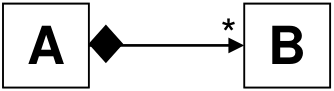
\includegraphics[width=1.0\textwidth]{figures/composite.png}
      \end{figure}
    \end{minipage}
    \begin{minipage}[t]{0.5\textwidth}
    \vspace{-3.5em}
    B is a fixed part of A that is:
    \begin{itemizenosep}
        \item B may be part of only one A
        \item If A is deleted, then also all its part
        \item Whole acts substitutions for all its parts\\
      $\Rightarrow$ operations are propagate to its parts
    \end{itemizenosep}
    \end{minipage}
  \end{defn}
\end{defnbox}
\begin{notebox}[Example]\nospacing
    House (parent) and a room (child), if we delete the house the
    room will be gone as well.
\end{notebox}
\begin{defnbox}\nospacing
  \begin{defn}[Aggregate]\label{defn:Aggregate}\leavevmode
    \begin{minipage}[t]{0.45\textwidth}
      \begin{figure}[H]
        \centering
        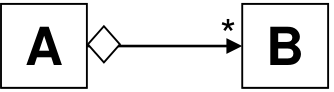
\includegraphics[width=1.0\textwidth]{figures/aggregate.png}
      \end{figure}
    \end{minipage}
    \begin{minipage}[t]{0.5\textwidth}
    \vspace{-3.5em}
    B is a variable part of A that is:
    \begin{itemizenosep}
        \item B may be part of several A's
        \item B may exist individually
    \end{itemizenosep}
    \end{minipage}
  \end{defn}
\end{defnbox}
\begin{notebox}[Example]\nospacing
    Class (parent) and Student (child), if we delete the class the
    students wills still exists, plus a student can be part of multiple classes.
\end{notebox}
\begin{figure}[H]
  \centering
  \vspace{-1em}
  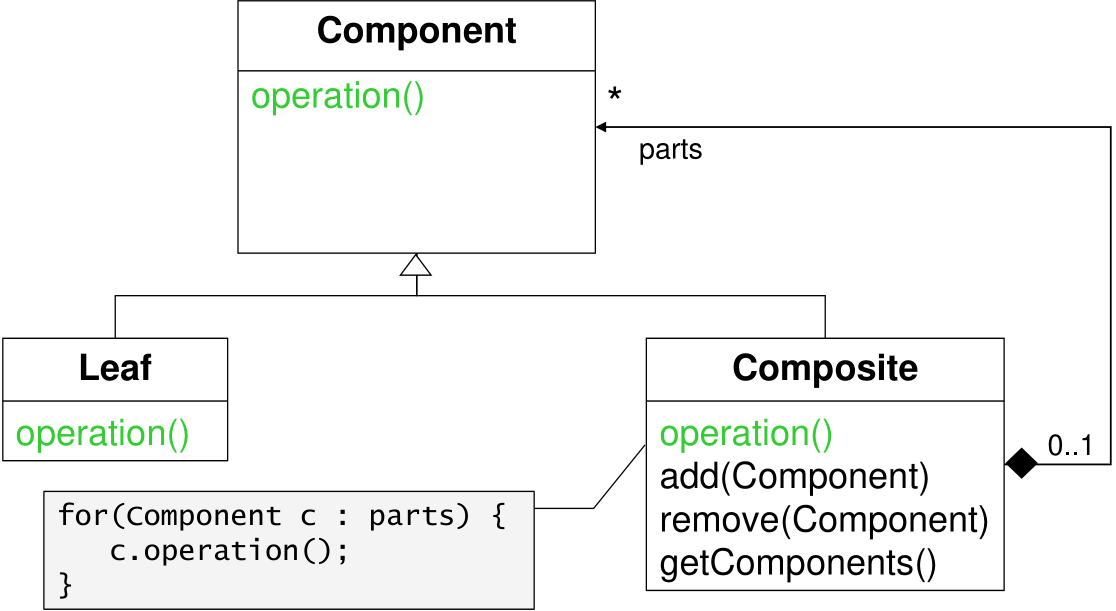
\includegraphics[width=1.0\columnwidth]{figures/compositePattern.png}
\end{figure}
\begin{intentbox}[Intent]
  Represent single/primitive components as hierarchical group such that we can treat
  the group object/composite the same way as the single objects.\\
  \imp{Examples} of operations applied uniformly on composites and single objects:
  \begin{itemize}
      \item Jdraw: move, draw, resize, copy
      \item File sizes: getSize, setProperties, delet
  \end{itemize}
\end{intentbox}
\begin{partbox}[Paticipants]
  \begin{itemizenosep}
      \item \imp{Abstract Class/Interface Component}: declares the base class
    and uniform methods implemented by the leaf primitives\\
      \imp{E.g.}\ Figure, Graphic, Shape, Room, ArithmeticOperation
      \item \imp{Leaves/primitives}: implements the Component interface/base class and
    specifies the behavior of the concrete primitive types\\
      \imp{E.g.}\ Rectangle, Text, Circle, PlayRoom, Multiply
      \item \imp{Composite}: implements the Component interface/base class and
      \begin{itemizenosep}
          \item Stores references to children which may be
          \begin{itemize}
              \item Leaves/Primitives
              \item Again composites
          \end{itemize}
          \item Implements methods to manage children add, remove, get
          \item Defines behavior of components containing children and must be
          concurrent with behavior of single elements
      \end{itemizenosep}
      \imp{E.g.} FigureGroup, GraphicsComposite, House,\\ ArithmeticExpression
        \item Client: manipulates objects through the Component interface
  \end{itemizenosep}
\end{partbox}
\subsection*{Transparent vs. Safe}
\label{subsubsec:TransparentVsSafe}
\begin{sectionbox}[Question]\nospacing
  Where should we \text{declare} the methods for managing the children, add, remove,\ldots?
  \begin{itemizenosep}
      \item \rdb{Transparent Approach}: declare them inside the Component
    interface
      \item \imp{\tc{Blue}{Safe Approach}}: declare them only inside the Composite
  \end{itemizenosep}
  \begin{figure}[H]
    \centering
    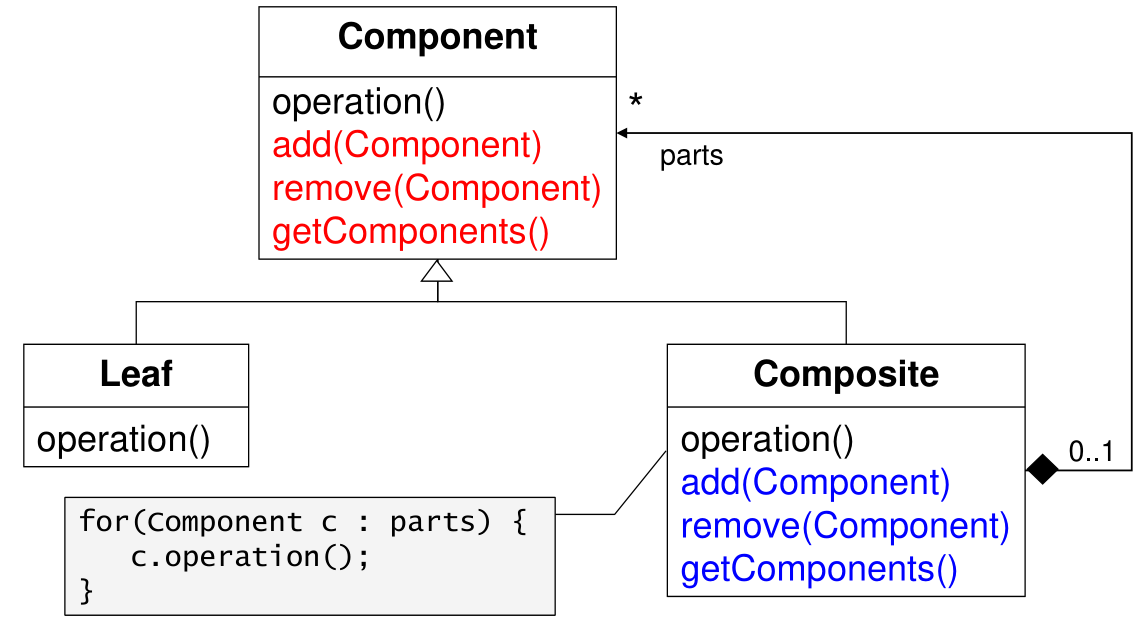
\includegraphics[width=1.0\textwidth]{figures/transSafe.png}
  \end{figure}
\end{sectionbox}
\subsubsection{\tc{Red}{Safe Approach \blackrb{Composite}}}
\begin{sectionbox}\nospacing
 Clients cannot do stupid/meaningless things s.a.\ adding, removing,\ldots from
 primitives/leaf objects because they do not even implement those methods
 $\Rightarrow$ compile time warning.
\end{sectionbox}
\todo[inline]{Understand what the drawback is with cast and treating uniformly}
\subsubsection{\tc{Blue}{Transparent Approach \blackrb{Component}}}
\begin{sectionbox}\nospacing
  Is the desire to treat composites and primitives uniformly/the same
  way/atomically/transparent and requires that we declare the child managing
  function inside the Component $\Rightarrow$ also the primitives must implement
  them $\Rightarrow$ clients may possibly do stupid things like adding to
  primitives.
\end{sectionbox}
\begin{sectionbox}[Solution 1]\nospacing
  Child managing methods inside the primitive throw an
  UnsupportedOperationException.\\
  \imp{Drawbacks}:
  \begin{itemizenosep}
      \item Program flow should not be controlled with exceptions
      \item Only transparent on the interface level
  \end{itemizenosep}
\end{sectionbox}
\begin{codeboxNl}{java}
  public void add|\optc{/}|remove(Component c ){
    throw new UnsupportedOperationException();
  }
 
  public void getComponents(){
    throw new UnsupportedOperationException();
  }
\end{codeboxNl}
\begin{sectionbox}[Solution 2]\nospacing
  Methods return a \javainline{boolean} result which informs the client whether
  the operation was successful.\\
  For \javainline{getComponents()} we can use
  \javainline{getComponents().getSize()} to check whether the composite contains
  components or not.
\end{sectionbox}
\begin{codeboxNl}{java}
  public boolean add(Component c) { return false; }
  public boolean remove(Component c) { return false; }
  public List getComponents() {return Collections.EMPTY_LIST;}
\end{codeboxNl}
\begin{sectionbox}[Solution 3]\nospacing
Method \javainline{isComposite} can be used to check whether a component is a
composite or not.\\
$\Rightarrow$ \javainline{isComposite()} should be called as precondition to
check if component is a composite, before add/remove,\ldots
\end{sectionbox}
\begin{codeboxNl}{java}
  public boolean isComposite() { return false; }
  public void add(Component c) { throw new AssertionError(); }
  public void remove(Component c){throw new AssertionError();}
  public List getComponents() {return Collections.EMPTY_LIST;}
\end{codeboxNl}
\begin{sectionbox}[Solution 4]\nospacing
  Default behavior is that nothing is done
\end{sectionbox}
\begin{codeboxNl}{java}
  public void add(Component c) {    /* do nothing */ }
  public void remove(Component c) { /* do nothing */ }
  public List getComponents() {return Collections.EMTPY_LIST;}
\end{codeboxNl}
\begin{sectionbox}[Solution 5]\nospacing
  Implement full functionality, that primitives can add and remove,\ldots
\end{sectionbox}
\subsection{Issues}
\begin{codeboxNl}[0..1 Constraint]{java}
  Figure f1 = new RectangleFigure(|\optldots|);
  Figure f2 = new RectangleFigure(|\optldots|);
  Figure f3 = new OvalFigure(|\optldots|);

  GroupFigure g1 = new GroupFigure(|\ul{f1}|, f2);
  GroupFigure g2 = new GroupFigure(f3, |\ul{f1}|);
\end{codeboxNl}
\begin{codeboxNl}[0..1 Constraint]{java}
  Figure f1 = new RectangleFigure(|\optldots|);
  Figure f2 = new RectangleFigure(|\optldots|);
  Figure f3 = new OvalFigure(|\optldots|);

  GroupFigure |\ul[ulc2]{g1}| = new GroupFigure(f1, f2);
  GroupFigure |\ul[ulc3]{g2}| = new GroupFigure(|\ul[ulc2]{g1}|, f3);

  |\ul[ulc2]{g1}|.addFigure(|\ul[ulc3]{g2}|);  // recursion
\end{codeboxNl}
\begin{sectionbox}[Solutions]\nospacing
  There exists to solutions:
  \begin{itemizenosep}
      \item \imp{Variant 1}: Only add component if it does not belong to anything:\\
      Check first for 0..1 constraint and then for recursion
      \item \imp{Variant 2}: If component belongs already to a composite remove it
      from current parent and add it to this composite.\\
      Check first for \ul[ulc4]{recursion} and then for 0..1 constraint
  \end{itemizenosep}
  in order to do this components need to have a parent field in order to check
  for recursions:
  \begin{mintlinebox}{java}
		Component parent;
  \end{mintlinebox}
\end{sectionbox}
\begin{codeboxNl}[Variant 1]{java}
void add(Component c) {
  // 1. Check 0..1 constraint
  if(c.parent != null) {
    throw new IllegalArgumentException("constraint violation");
  }
  // => c is for sure not part of anything
  // But c maybe composite itself 

  // 2. Check for recursion 
  // c has no parents => only possibility for recursion if
  // c is the same as root of this
  if(c instanceof Composite) {
    Composite comp = this;
    while (|\uldotted{comp.parent != null}|) { comp = comp.parent; }
    if(comp == c) {
      throw new IllegalArgumentException("recursion");
    }
  }

  c.parent = this;
  this.children.add(c);
}
\end{codeboxNl}
\begin{notebox}[Note]\nospacing
  Recursion only possible if \javainline{c} is the same as
  root of \javainline{this}. Root because we already know that
  \uldotted{\javainline{c} has not parent}.
\end{notebox}
\begin{codeboxNl}[Variant 2]{java}
void add(Component c) {
  // 1. Check for recursion
  // recursion not possible if c is primitive
  if(c instanceof Composite) {
    Composite comp = this;
    while (comp != null && comp != c) { comp = comp.parent; }
    // |go up in the hierarchy check for recursion
      if(|\ul[ulc4]{comp == c}|) {
        throw new IllegalArgumentException("recursion");
      }
    }

  // 2. Establish 0..1 constraint
  if(c.parent != null) {
    c.parent.remove(c);
  }

  c.parent = this;
  this.children.add(c);
}
\end{codeboxNl}
%%% Local Variables:
%%% mode: latex
%%% TeX-master: "../formulary"
%%% End:
